% --------------------------------------------------------------
% This is all preamble stuff that you don't have to worry about.
% Head down to where it says "Start here"
% --------------------------------------------------------------

\documentclass[11pt]{article}
\usepackage[margin=1in]{geometry}
\usepackage{amsmath,amsthm,amssymb}
%\usepackage{multicol}
\usepackage{graphicx}
%\usepackage{fixltx2e}
%\usepackage{amsmath}

\usepackage{tikz}
\usepackage{pgfplots}
\usepackage{fourier}
\usepackage[inline]{enumitem}
\usepackage{subcaption}



%\everymath{\displaystyle}

\newcommand\ft{Fourier transform}
\newcommand\ift{inverse Fourier transform}
\newcommand\ftr{Fourier transform representation}
\newcommand\fs{Fourier series}
\newcommand\fsr{Fourier series representation}
\newcommand\xt{$x(t)$}
\newcommand\xo{$X(j\omega)$}

\title{\Large Department of Electronic and Telecommunication Engineering\\University of Moratuwa\\Sri Lanka\\{\LARGE \bf \textsc{EN1060 Signals and Systems: Tutorial 03 \footnote{All the questions are from Oppenheim \emph{et al.} chapter 4.}}}}

\date{\vspace{-0.2in}\today}


\newcommand{\N}{\mathbb{N}}
\newcommand{\Z}{\mathbb{Z}}

\begin{document}



\maketitle
\noindent \tikz \draw (0,0) -- (\textwidth,0);

\begin{enumerate}
    % Q01 Oppenheim et al. 4.1
    \item Use the \ft~ analysis equation to calculate the \ft{}s of
        \begin{enumerate}
            \item $e^{-2(t-1)}u(t-1)$
            \item $e^{-2|t-1|}$
        \end{enumerate}
    % Q02 Oppenheim et al. 4.2
    \item Use the \ft~ analysis equation to calculate the \ft{}s of
        \begin{enumerate}
            \item $\delta(t+1) + \delta(t-1)$
            \item $\frac{d}{dt}[u(-2-t) + u(t-2)]$
        \end{enumerate}
        Sketch and label the magnitude of each \ft.
    % Q03 Oppenheim et al. 4.3
    \item Determine the \ft~ of each of the following periodic signals:
        \begin{enumerate}
            \item $\sin(2\pi t+ \pi/4)$
            \item $1 + \cos(6\pi t+ \pi/8)$
        \end{enumerate}
    % Q04 Oppenheim et al. 4.4
    \item Use the \ft~ synthesis equation to determine the \ift~of
        \begin{enumerate}
            \item $X_1(j\omega) = 2\pi\delta(\omega) + \pi \delta(\omega - 4\pi) + \pi \delta(\omega + 4\pi)$
            \item $X_2(j\omega) = \begin{cases}2, & 0\leq \omega \leq 2, \\-2, & -2 \leq \omega <0,\\ 0, & |\omega| > 2.\end{cases}$
        \end{enumerate}
    % Q05 Oppenheim et al. 4.5
    \item Use the \ft~ synthesis equation to determine the \ift~of  $X(j\omega) = |X(j\omega)|e^{j\angle X(j\omega)}$ where
    \begin{align*}
      |X(j\omega)| &= 2[u(\omega + 3)-u(\omega -3)] \\
      \angle X(j\omega) &= -\frac{3}{2}\omega + \pi\\
    \end{align*}


    % Q21 Oppenheim et al. 4.21
    \item  \label{qu:17} Compute the \ft~of each of the following signals:
    \begin{enumerate}
        \item $[e^{-\alpha t} \cos \omega_0 t]u(t),\quad \alpha >0$
        \item $e^{-3|t|} \sin 2t \omega_0 t$
        \item $x(t) = \begin{cases}1 + \cos \pi t,& |t| <1\\ 0, & |t|>1\end{cases}$
        \item $\sum_{k=0}^{\infty} \alpha^k \delta(t - kT), \quad |\alpha| < 1$
        \item  $[te^{-2 t} \sin  4t]u(t)$
        \item $\left[\frac{\sin \pi t}{\pi t}\right]\left[\frac{\sin 2\pi (t-1)}{\pi (t-1)}\right]$
        \item $x(t)$ as shown in Figure \ref{sfi:q17a}.
        \item $x(t)$ as shown in Figure \ref{sfi:q17b}.
    \end{enumerate}

    \begin{figure}
      \centering
        \begin{subfigure}[t]{0.3\textwidth}
            \centering
            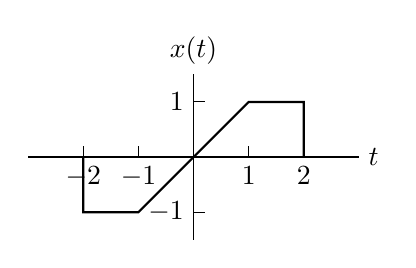
\begin{tikzpicture}[scale=0.70]
	\draw (-3,0) -- (3,0) node[anchor=west] {$t$};
	\draw (0, -1.5) -- (0,1.5) node[anchor=south] {$x(t)$};	
	\foreach \x in {-2, -1, 1, 2}
	{
		\draw (\x, 0.2) -- ++(0, -0.2);
		\node at (\x, 0) [anchor=north ] {$\x$};
	}
	\foreach \y in {-1, 1}
	{
		\draw (0.2, \y) -- ++(-0.2, 0);
		\node at (0, \y) [anchor=east ] {$\y$};
	}	
	
	\draw[thick] (-2, 0) |- (-1, -1)  -- (1,1) -| (2,0);
\end{tikzpicture} 
            \caption{}\label{sfi:q17a}
        \end{subfigure}%
        \hfill
        \begin{subfigure}[t]{0.7\textwidth}
            \centering
            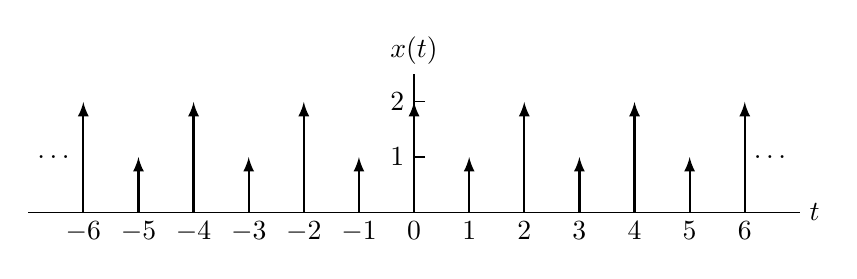
\begin{tikzpicture}[scale=0.70]
	\draw (-7,0) -- (7,0) node[anchor=west] {$t$};
	\draw (0, 0) -- (0,2.5) node[anchor=south] {$x(t)$};	
	\foreach \x in {-6, -5, ..., 6}
	{
		\draw (\x, 0.2) -- ++(0, -0.2);
		\node at (\x, 0) [anchor=north ] {$\x$};
	}
	\foreach \y in {1,2}
	{
		\draw (0.2, \y) -- ++(-0.2, 0);
		\node at (0, \y) [anchor=east ] {$\y$};
	}	
	
	\foreach \x in {-6, -4, ..., 6}
	{
		\draw[thick, latex-] (\x, 2) -- ++(0, -2);
	}
	
	\foreach \x in {-5, -3, ..., 5}
	{
		\draw[thick, latex-] (\x, 1) -- ++(0, -1);
	}	
	
	\node at (-6.5, 1) {\dots};
	\node at (6.5, 1) {\dots};
	
\end{tikzpicture} 
            \caption{}\label{sfi:q17b}
        \end{subfigure}
      \caption{Figure for Q\ref{qu:17}}\label{fi:q17}
    \end{figure}


    % Q22 Oppenheim et al. 4.22
    \item  \label{qu:18} Determine the continuous-time signal corresponding to each of the following transfroms:
    \begin{enumerate}
      \item $X(j\omega) = \dfrac{2\sin[3(\omega - 2\pi)]}{\omega - 2\pi}$
      \item $X(j\omega) = \cos(4\omega + \pi/3)$
      \item $X(j\omega)$ as given in the magnitude and phase plots of Figure \ref{sfi:q18a}
      \item $X(j\omega) = 2[\delta(\omega -1) - \delta(\omega + 1)] + 3[\delta(\omega -2\pi) + \delta(\omega + 2\pi)]$
      \item $X(j\omega)$ as  in Figure \ref{sfi:q18b}
    \end{enumerate}

    \begin{figure}
      \centering
        \begin{subfigure}[t]{0.3\textwidth}
            \centering
            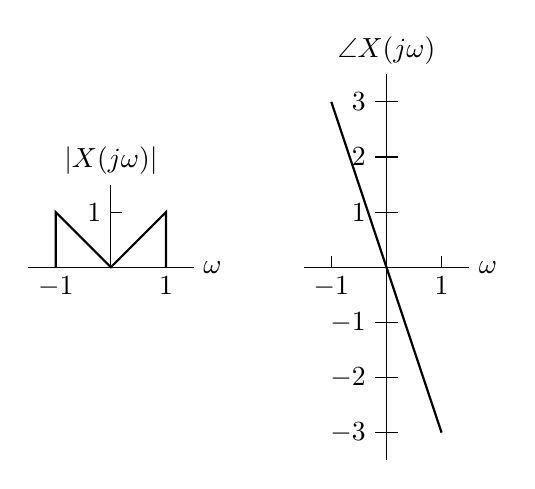
\begin{tikzpicture}[scale=0.70]
	\begin{scope}
		\draw (-1.5,0) -- (1.5,0) node[anchor=west] {$\omega$};
		\draw (0, 0) -- (0,1.5) node[anchor=south] {$|X(j\omega)|$};	
		\foreach \x in {-1, 1}
		{
			\draw (\x, 0.2) -- ++(0, -0.2);
			\node at (\x, 0) [anchor=north ] {$\x$};
		}
		\foreach \y in {1}
		{
			\draw (0.2, \y) -- ++(-0.2, 0);
			\node at (0, \y) [anchor=east ] {$\y$};
		}	
		
		\draw[thick] (-1,0) -- (-1,1) -- (0,0) -- (1,1) -- (1,0);
	\end{scope}
	\begin{scope}[xshift=5cm]
		\draw (-1.5,0) -- (1.5,0) node[anchor=west] {$\omega$};
		\draw (0, -3.5) -- (0,3.5) node[anchor=south] {$\angle X(j\omega)$};	
		\foreach \x in {-1, 1}
		{
			\draw (\x, 0.2) -- ++(0, -0.2);
			\node at (\x, 0) [anchor=north ] {$\x$};
		}		

		\foreach \y in {-3,-2, -1, 1, 2, 3}
		{
			\draw (0.2, \y) -- ++(-0.4, 0) node [anchor=east ] {$\y$};
		}	
		
		\draw[thick] (-1,3) -- (1,-3);
	\end{scope}	

	
\end{tikzpicture} 
            \caption{}\label{sfi:q18a}
        \end{subfigure}%
        \hfill
        \begin{subfigure}[t]{0.7\textwidth}
            \centering
            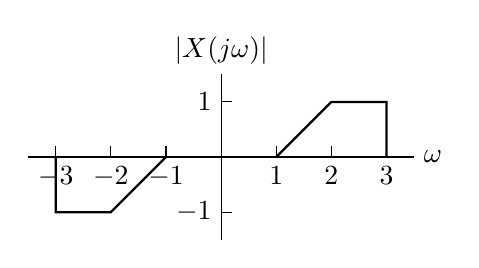
\begin{tikzpicture}[scale=0.70]
	\begin{scope}
		\draw (-3.5,0) -- (3.5,0) node[anchor=west] {$\omega$};
		\draw (0, -1.5) -- (0,1.5) node[anchor=south] {$|X(j\omega)|$};	
		\foreach \x in {-3, -2, -1, 1, 2, 3}
		{
			\draw (\x, 0.2) -- ++(0, -0.2);
			\node at (\x, 0) [anchor=north ] {$\x$};
		}
		\foreach \y in {-1, 1}
		{
			\draw (0.2, \y) -- ++(-0.2, 0);
			\node at (0, \y) [anchor=east ] {$\y$};
		}	
		
		\draw[thick] (-3,0) |- (-2, -1) -- (-1,0) (1,0) -- (2,1) -| (3,0); 
	\end{scope}
	
\end{tikzpicture} 
            \caption{}\label{sfi:q18b}
        \end{subfigure}
      \caption{Figure for Q\ref{qu:18}}\label{fi:q181}
    \end{figure}

    % Q06 Oppenheim et al. 4.6
    \item Given that \xt~ has the \ft~ \xo, express the \ft s of the signals listed below in terms of \xo. You may find useful the \ft~properties listed in the table in the book.
        \begin{enumerate}
            \item $x_1(t) = x(1-t) + x(-1-t)$
            \item $x_2(t) = x(3t-6) $
            \item $x_3(t) = \frac{d^2}{dt^2}x(t-1) $
        \end{enumerate}
    % Q07 Oppenheim et al. 4.7
    \item For each of the following \ft s, use \ft~ properties to determine whether the corresponding time-domain signal is (i) real, imaginary, or neither and (ii) even, odd, or neither. Do this without evaluating the given transforms.
        \begin{enumerate}
            \item $X_1(j\omega) = u(\omega) - u(\omega -2)$
            \item $X_2(j\omega) = \cos(2\omega)\sin(\omega/2)$
            \item $X_3(j\omega) = A(\omega)e^{jB(\omega)}$ where $A(\omega) = (\sin 2\omega)/\omega$ and $B(\omega) = 2\omega + \pi/2$
            \item $X_4(j\omega) = \sum_{k=-\infty}^{\infty}\left(\frac{1}{2}\right)^{|k|}\delta\left(\omega - \frac{k\pi}{4}\right)$
        \end{enumerate}
    % Q08 Oppenheim et al. 4.8
    \item Consider the signal
        \begin{equation*}
            x(t) = \begin{cases} 0, & t < \frac{1}{2},\\ t + \frac{1}{2}, & -\frac{1}{2} \leq t \leq \frac{1}{2},\\1, & t>\frac{1}{2}.
            \end{cases}
        \end{equation*}
        \begin{enumerate}
            \item Use differentiation and integration properties and the \ft~ pair for the rectangular pulse to find a closed-form expression for \xo.
            \item What is the \ft~ of $g(t) = x(t) - \frac{1}{2}$?
        \end{enumerate}
    % Q09 Oppenheim et al. 4.9
    \item Consider the signal
        \begin{equation*}
            x(t) = \begin{cases} 0, & |t| > 1,\\ (t + 1)/2, & -1 \leq t \leq 1.\end{cases}
        \end{equation*}
        \begin{enumerate}
            \item With the help of tables, determine the closed-form expression for \xo.
            \item Take the real part of your answer above, and verify that it is the \ft~ of the even part of \xt.
            \item What is the \ft~ of the odd part of \xt?
        \end{enumerate}

    % Q10 Oppenheim et al. 4.10
    \item
        \begin{enumerate}
            \item Use tables to help determine the \ft~ of the following signal:
            \begin{equation*}
                x(t) = t\left(\frac{\sin t}{\pi t}\right)^2.
            \end{equation*}
            \item Use Pasrseval's relation and the result of the previous part to determine the numerical value of
            \begin{equation*}
                A = \int_{-\infty}^{\infty} t^2\left(\frac{\sin t}{\pi t}\right)^4.
            \end{equation*}
        \end{enumerate}

    % Q11 Oppenheim et al. 4.11
    \item Given the relationship
    \begin{equation*}
        y(t) = x(t)\ast h(t),
    \end{equation*}
    and
    \begin{equation*}
        g(t) = x(3t)\ast h(3t),
    \end{equation*}
    and given that \xt~has \ft~ \xo~and $h(t)$ has \ft~ $H(j\omega)$, use \ft~ properties to show that $g(t)$ has the form
    \begin{equation*}
        g(t) = Ay(Bt).
    \end{equation*}
    Determine the values of $A$ and $B$.

    % Q12 Oppenheim et al. 4.12
    \item Consider the \ft~pair
    \begin{equation*}
        e^{-|t|} \overset{\mathcal{F}}{\longleftrightarrow} \frac{2}{1+\omega^2}.
    \end{equation*}
    \begin{enumerate}
        \item Use the appropriate \ft~properties to find the \ft~of $te^{-|t|}$.
        \item Use the result from part (a), along with the duality property, to determine the \ft~of
        \begin{equation*}
          \frac{4t}{(1+t^2)^2}.
        \end{equation*}
    \end{enumerate}
    \emph{Hint:} See \ref{qu:q13}.

    % Q13 Oppenheim et al. 4.13
    \item \label{qu:q13}.Let \xt~be a signal whose \ft~is
    \begin{equation*}
        X(j\omega) =\delta(\omega)+\delta(\omega -\pi) + \delta(\omega-5),
    \end{equation*}
    and let
    \begin{equation*}
        h(t) = u(t) - u(t-2).
    \end{equation*}
    \begin{enumerate}
        \item Is \xt~periodic?
        \item Is $x(t)\ast h(t)$ periodic?
        \item Can the convolution of two aperiodic signals be periodic?
    \end{enumerate}

    % Q14 Oppenheim et al. 4.14
    \item  Consider a signal \xt~with \ft~\xo. Suppose we are given the following facts:
    \begin{enumerate}
        \item \xt~is real and non-negative.
        \item $\mathcal{F}^{-1}{(1+j\omega)X(j\omega)} = Ae^{-2t}u(t)$, where $A$ is independent of $t$.
        \item $\int_{-\infty}^{\infty}|X(j\omega)|^2d\omega = 2\pi$.
    \end{enumerate}
    Determine a closed-form expression for \xt.

    % Q15 Oppenheim et al. 4.15
    \item  Let \xt~be a signal with \ft~\xo. Suppose we are given the following facts:
    \begin{enumerate}
        \item \xt~is real.
        \item $x(t)=0$ for $t\leq 0$.
        \item $\frac{1}{2\pi}\int_{-\infty}^{\infty}\mathfrak{Re} \{ X(j\omega)\}e^{j\omega t}d\omega = |t|e^{-|t|}$.
    \end{enumerate}
    Determine a closed-form expression for \xt.

    % Q16 Oppenheim et al. 4.16
    \item Consider the signal
    \begin{equation*}
        x(t) = \sum_{-\infty}^{\infty}\frac{\sin\left(k\frac{\pi}{4}\right)}{k\frac{\pi}{4}}\delta\left(t - k\frac{\pi}{4}\right).
    \end{equation*}
    \begin{enumerate}
        \item Determine $g(t)$ such that
        \begin{equation*}
            x(t) = \left(\frac{\sin t}{\pi t}\right)g(t).
        \end{equation*}
        \item Use the multiplication property of the \ft~ to argue that \xo~is periodic. Specify \xo~over one period.
    \end{enumerate}

    % Q19 Oppenheim et al. 4.37
   \item \label{qu:437} Consider the signal \xt~in Figure \ref{fi:q437}.
   \begin{enumerate}
        \item Find the \ft~\xo~of \xt.
        \item Sketch the signal
        \begin{equation*}
          \tilde{x}(t) = x(t)\ast \sum_{k = -\infty}^{\infty}\delta(t-4k).
        \end{equation*}
        \item Find another signal $g(t)$ such that $g(t)$ is not the same as \xt~and
        \begin{equation*}
          \tilde{x}(t) = g(t)\ast \sum_{k = -\infty}^{\infty}\delta(t-4k).
        \end{equation*}
        \item Argue that, although $G(j\omega)$ is different from \xo,   $G(j\frac{\pi k}{2}) = X(j\frac{\pi k}{2})$   for all integers $k$. You should explicitly evaluate  $G(j\omega)$ to answer this question.
   \end{enumerate}
    \begin{figure}
      \centering
      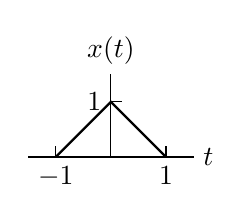
\begin{tikzpicture}[scale=0.70]
	\begin{scope}
		\draw (-1.5,0) -- (1.5,0) node[anchor=west] {$t$};
		\draw (0, 0) -- (0,1.5) node[anchor=south] {$x(t)$};	
		\foreach \x in {-1, 1}
		{
			\draw (\x, 0.2) -- ++(0, -0.2);
			\node at (\x, 0) [anchor=north ] {$\x$};
		}
		\foreach \y in {1}
		{
			\draw (0.2, \y) -- ++(-0.2, 0);
			\node at (0, \y) [anchor=east ] {$\y$};
		}	
		
		\draw[thick] (-1,0) -- (0,1) -- (1,0); 
	\end{scope}
	
\end{tikzpicture} 
      \caption{Figure for Q\ref{qu:437}}\label{fi:q437}
    \end{figure}

    % Q20 Oppenheim et al. 4.38
    \item Let \xt~be any signal with \ft~\xo. The frequency-shift property of the
    ft~may be stated as
    \begin{equation*}
        e^{j\omega_0 t} \overset{\mathcal{F}}{\longleftrightarrow}  X(j(\omega - \omega_0)).
    \end{equation*}
    \begin{enumerate}
        \item Prove the frequency-shift property by applying the frequency shift to the analysis equation
        \begin{equation*}
            X(j\omega) = \int_{-\infty}^{\infty}x(t)e^{-j\omega t}dt.
        \end{equation*}
        \item Prove the frequency-shift property by utilizing the \ft~of $e^{j\omega_0 t}$ in conjunction with the multiplication property of the \ft.
    \end{enumerate}
\end{enumerate}
\end{document} 